\documentclass{article}
\usepackage{graphicx}


\begin{document}

asdasdasd

\section{lalal}
\begin{figure}[htbp]
    \centering
    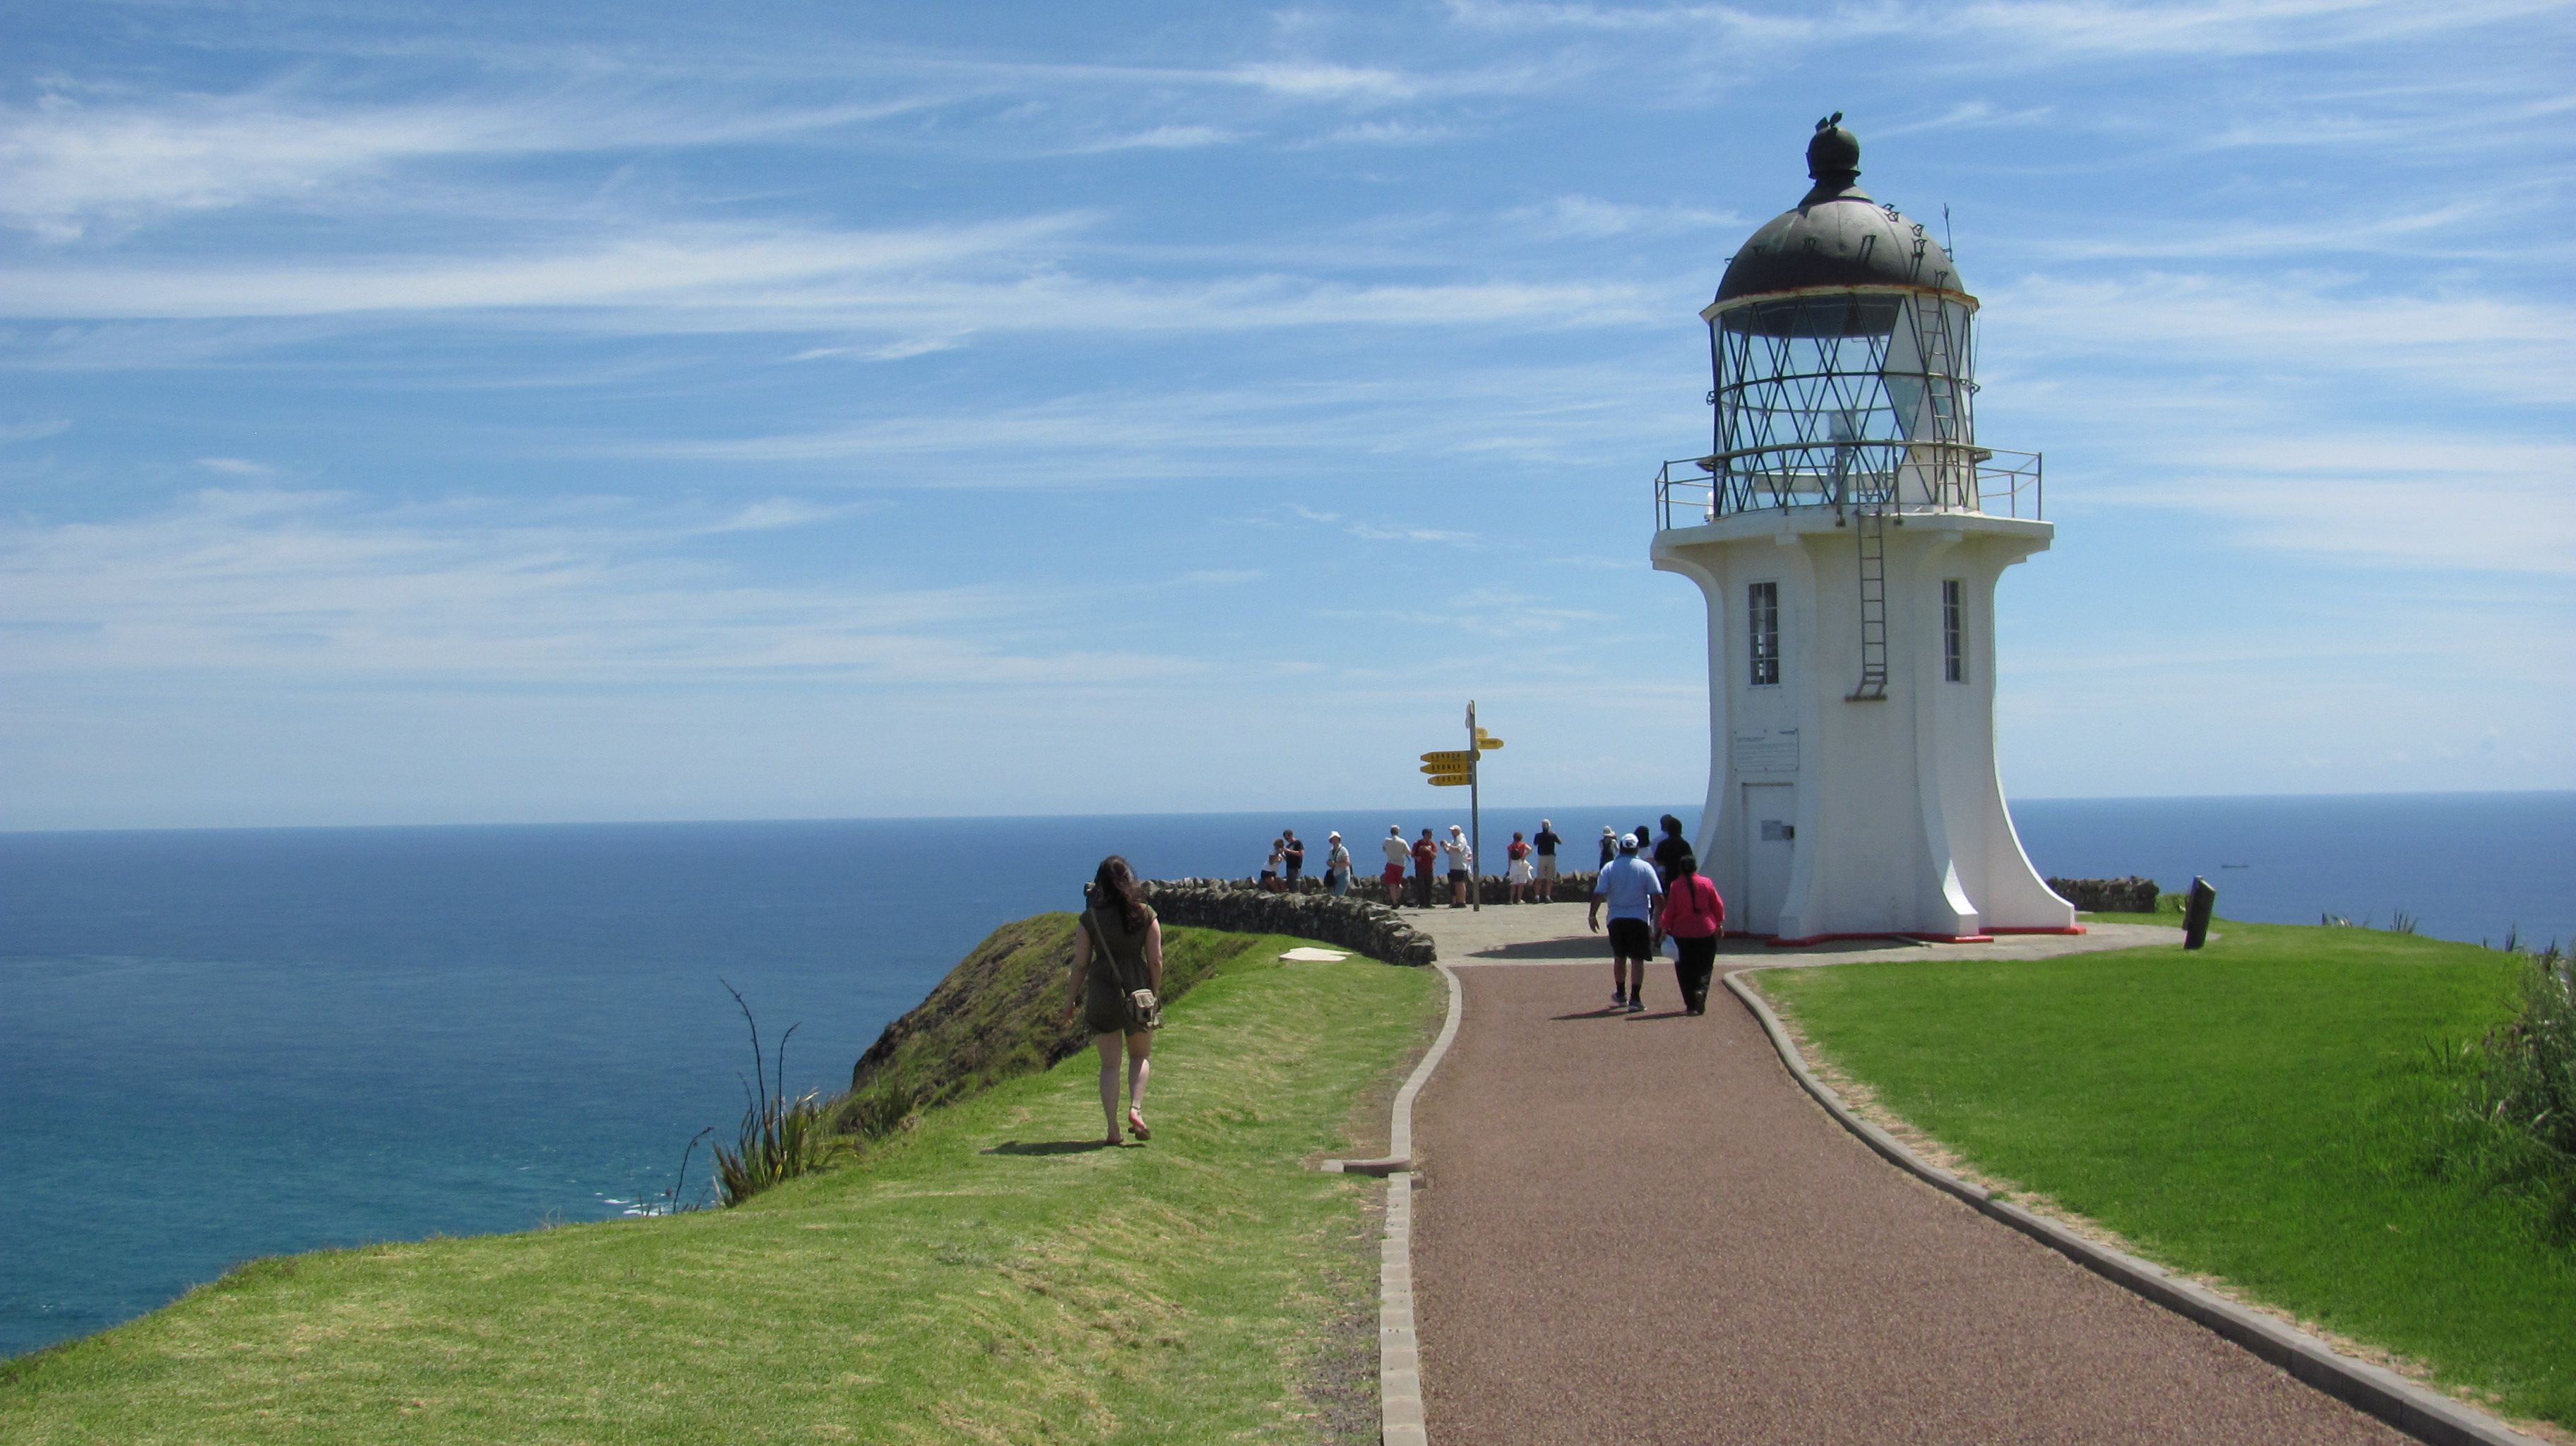
\includegraphics[width=.9\textwidth]{./image}
    \caption{Das Diagramm zeigt die zurueckgelegte Strecke nach einer bestimmten Zeit.}
    \label{fig:st-diag}
\end{figure}

\begin{eqnarray}
f(x) & := & x^2 \\
f( 0 )  &=&  0 \nonumber\\
f( 1 )  &=&  1 \nonumber\\
f( 2 )  &=&  4 \nonumber\\
f( 3 )  &=&  9 \nonumber\\
f( 4 )  &=&  16 \nonumber\\
f( 5 )  &=&  25 \nonumber\\
f( 6 )  &=&  36 \nonumber\\
f( 7 )  &=&  49 \nonumber\\
f( 8 )  &=&  64 \nonumber\\
f( 9 )  &=&  81 \nonumber\\
\end{eqnarray}


Das ist ein Beispiel.
\end{document}
